\chapter{実験}

\section{データ収集}

\subsection{配管画像の取得}
配管画像の取得には、大規模な配管設備に対する実験を行うため、シミュレーション環境で配管の画像を取得した。
また、配管画像の取得には、RGB-DカメラであるRealsense D435iとAzure Kinect DKを使用することを想定する。
図2には、RGB-Dカメラで撮影した配管画像の例と、シミュレーション環境で取得した画像の例を示した。

\subsection{センサーモデルの導入}
シミュレーション環境を実環境に近づけるため、Azure Kinect DKのセンサノイズを計測した。
0.5mから9.5mの範囲で0.5m間隔ごとに、実際の距離と測定距離の標準偏差を測定し、その結果を指数関数で近似した。
この近似結果をセンサーモデルとしてシミュレーションに導入した。図3は標準偏差をもとに近似した結果を示した。



% RGB-Dカメラから取得したデータセットをRXDネットワークを使用し曲管又はT字管を認識できるか検証する.
% 物体認識においては他のネットワークでも実験し,RXDネットワークの有用性を確かめる.
% また,物体検出から得た情報を曲管及びT字管の姿勢推定も行う.

% \section{使用機材}
% データセットの取得にはRGB-Dカメラを使用する.従来の方法ではLIDARセンサーを用いて配管3Dデータやアイソメ図を作成していた.
% しかし,LIDARセンサーは高価であり,一般的に使用することが困難であるという欠点を抱えていた.そのため,RGB-DカメラはLIDARセンサーよりも比較的安価であるため本研究のデータセット収集に使用する.\\
% 次に,RGBカメラではなくRGB-Dカメラを使用する利点を3点紹介する.まず,一つ目にRGB-Dカメラはカラー画像だけでなく距離情報を取得できるという点である.
% 配管のアイソメ図には配管のそれぞれの部位の長さを正確に示す必要がある.そのため,RGB画像には距離情報が含まれていないことからスケールを必要とする際にはDepth画像が重要になるのだ.\\
% 二つ目に照明などの光の明暗に影響されない点である.図3.2よりRGB画像は撮影する環境が照明が無く暗闇だった場合,撮影された画像には認識したいオブジェクトの特徴を捉えることは困難である.これはRGB画像が光に反射された物体の度合いを数値化しているため,極端に明るすぎたり
% 暗すぎるとRGB画像が活用できなくなる.特に配管が設置されている地盤地下や天井裏などの照明を当てることが困難な環境ではDepth画像が必要になる.\\
% \begin{figure}[htbt]
%     \centering
%      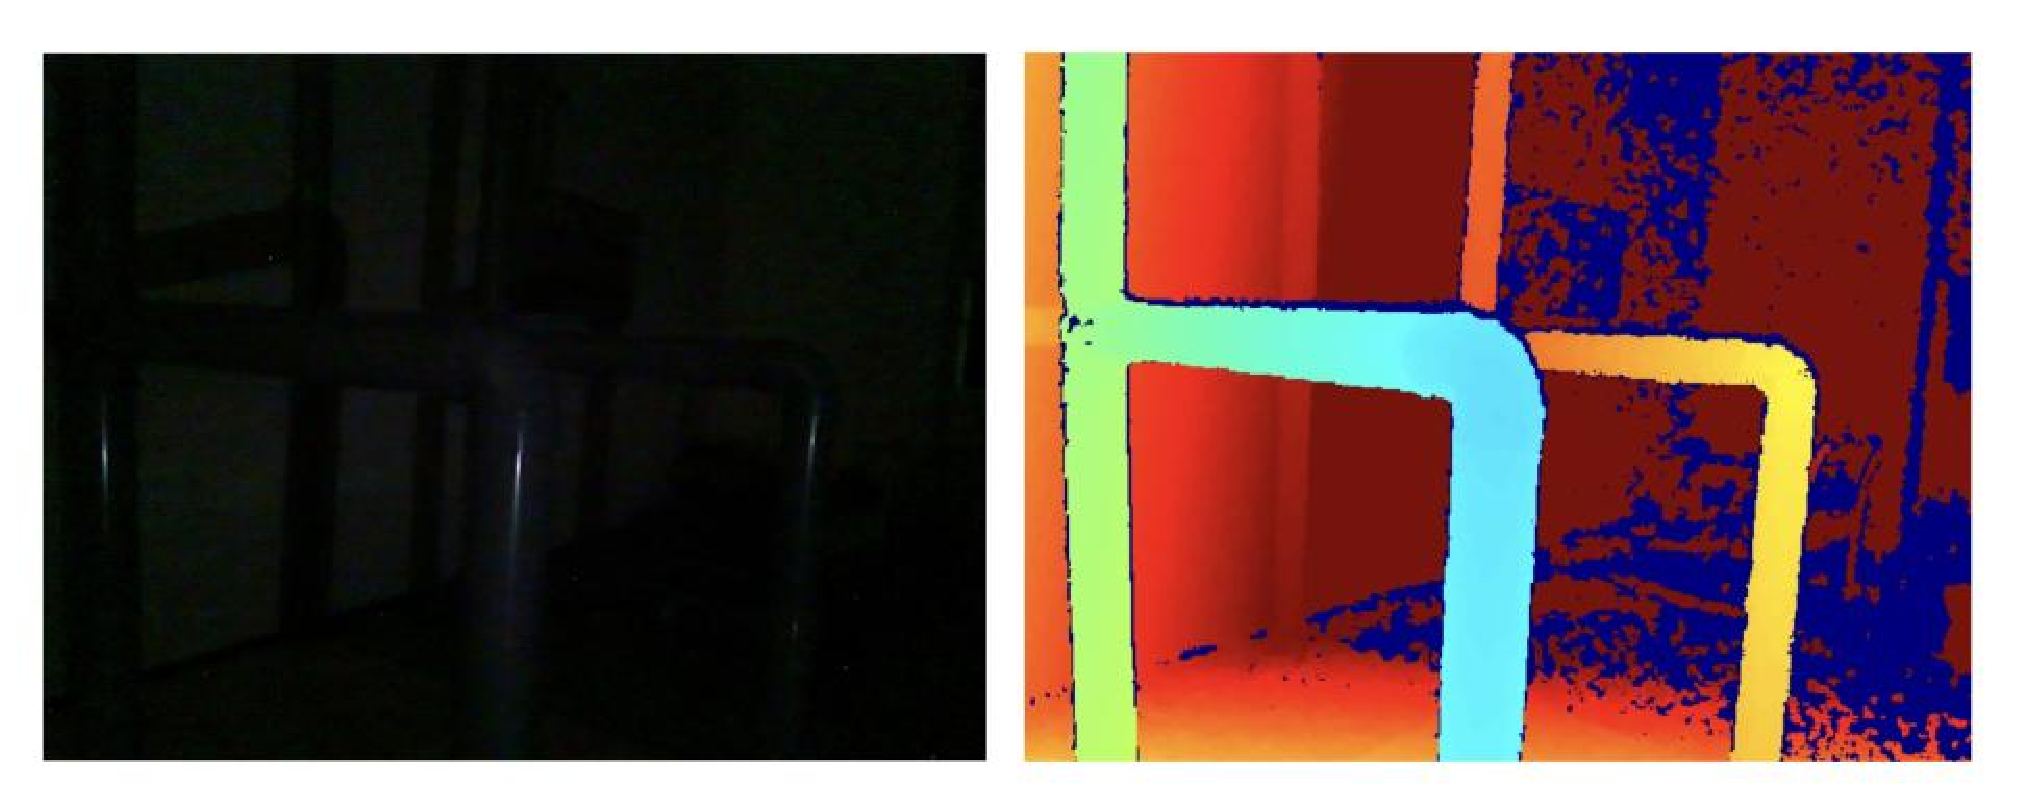
\includegraphics[height=45mm]{pipe_rgbd.eps}
%      \caption{暗所でのRGB-Dカメラの撮影}
%      \label{fig:f2}
% \end{figure}
% 三つ目に配管が背景色と同様の色を示していた場合に,区別が容易に可能であるという点である.RGB画像では色の違いの判断が難しいが,Depth画像は距離情報の違いを示すことができるため,
% 背景と異なる物体として認識可能になる.配管の場合,壁と配管の色に差異が生まれにくいことが多々あるためDepth画像を使用するメリットになる.また,配管が重なり合った場合にも前後関係が区別しない場合にも効果を発揮する.\\

% カメラはインテル社製のIntel Realsense L515を使用した.Realsense L515を使用した理由はRealsenseカメラの中でも屋内に適したRGB-Dカメラであるからだ.このカメラは外光の影響を受けやすいが,
% 屋内の環境であればその影響を受けないため,配管などの室内で多く使用される環境では非常に適していると判断した.
% \begin{figure}[htbt]
%     \centering
%      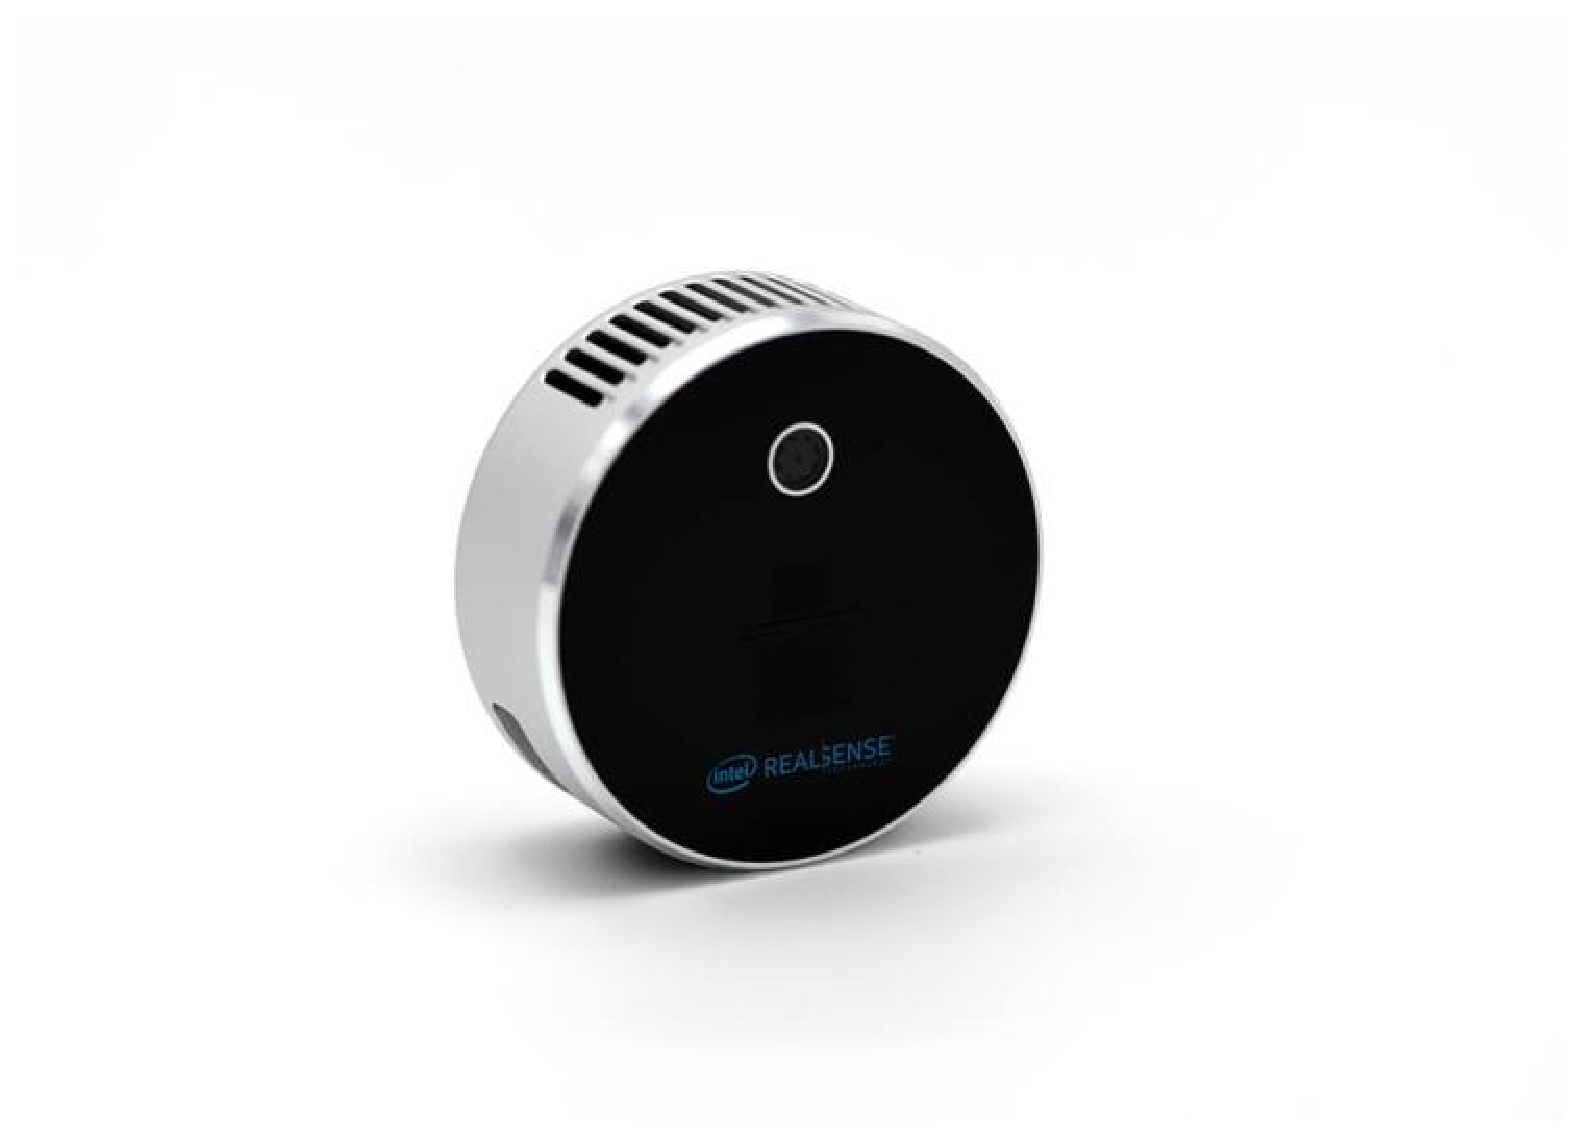
\includegraphics[height=65mm]{realsense.eps}
%      \caption{Intel Realsense L515}
%      \label{fig:f2}
% \end{figure}

% しかし,Realsense L515は仕様上,RGBカメラとDepthカメラの位置が異なるため,撮影した際に両方の画像を比較すると画角に差異が生じてしまう.これは,データセットのラベリングを行う際に配管のピクセル座標に
% それぞれの画像で異なると認識の精度に大きな誤差が生じてしまう.そのため,Realsenseのalignmentライブラリを使用する.これによって両方のカメラの画角をソフトウェア上で位置合わせが可能になる.

% \section{物体検出のデータセット収集}
% 深層学習による認識ネットワークにはデータセットの数量が多いほど精度とロバスト性が向上する.
% それは様々な場面での配管の写真を学習することによってどの環境においても対応できる汎用性が高まることを意味している.本研究使用するデータセットの一部を図3.2に示す.
% 配管には曲管やT字管や直管が含まれており,この画像内の中から曲管とT字管を全て認識できることを目標とする.また,Depth画像の有効性を示すためにテスト画像では
% 暗闇の中に配管を設置したデータセットを用意した.Depth画像は光の影響を受けにくいことから,暗闇の中でも配管を認識できるかを検証する.\\
% 収集したデータはラベリング作業を行う.これは深層学習するにおいての正解データとして,予め画像内のどの部分が曲管又はT字管であるかをアノテーションする必要がある.
% 本研究では配管画像に対して曲管,T字管の二つのクラスに分けてラベリング作業を行った.

% \begin{figure}[htbt]
% 	\centering
% 	 \includegraphics[height=155mm]{imges.eps}
% 	 \caption{学習に用いるデータセットの例}
% 	 \label{fig:f2}
% \end{figure}

% \section{6D姿勢推定のデータセット収集}
% 6D姿勢推定のデータセットにはColmapを使用して点群データを取得する.Colmap2D画像から点群を再構築するために使用されるソフトウェアである.
% この2D画像は異なる視点から撮影された同じオブジェクトの画像を複数枚利用することで3次元情報を復元することができる.
% そのため,本研究では曲管とT字管の周囲をそれぞれ撮影し,Colmapを使用することで点群データを取得した.
% 図3.6では姿勢推定を行った後,得られた出力の評価を行う際に使用する.
% しかし,点群データを取得してもColmapで生成されたデータには距離情報が含まれていないため,別途Depth画像を使用してアイソメ図作成の際に使用しなければいけない.
% \begin{figure}[htbt]
% 	\centering
% 	 \includegraphics[height=90mm]{bent.eps}
% 	 \caption{Colmapを用いた曲菅の点群データ}
% 	 \label{fig:f2}
% \end{figure}

% \begin{figure}[htbt]
% 	\centering
% 	 \includegraphics[height=95mm]{junction_p.eps}
% 	 \caption{Colmapを用いたT字管の点群データ}
% 	 \label{fig:f2}
% \end{figure}

% \clearpage
% \section{評価指標}
% 物体認識の評価指標ではパラメータ数(Params), Intersection over Union(IoU), mean Average Precision(mAP)を用い認識ネットワークの性能評価を行う.
% まず,パラメータ数は認識ネットワークの学習可能なパラメータの合計数を示す.これにより,認識ネットワークの複雑度を示すことができ,パラメータ数が多いほどネットワークが複雑になり推論字管が長くなるのが一般的である.
% 次に,IoUは図3.6のように正解ラベルと予測のバウンディングボックスの共通の重なり部分と,2つのバウンディングボックスを重ねたときの総面積で除算したものである.
% IoUは0~1.0の値の範囲で示され,値が大きければ大きいほどラベル付されたボックスと予測されたボックスの重なりが正しいことになり,正確に認識していると判断できる.\\
% 次に,mAPは一つ一つのクラスに対して平均適合率であるAP(Average Precision)を計算する.まず,モデルの予測結果を,出力する信頼度スコア順に並べる.
% ラベルごとに信頼度スコアがそのラベルの値以上の予測結果について,適合率と再現率を求める.適合率と再現率は図3.7のようにTrue Positive(TP)とFalse Negative(FN)を用いて表される.
% その適合率と再現率のグラフから適合率の下側の面積を求める.ここで,予測されたラベルが正解なのかの判断はIoUが決められたしきい値以上で,最も信頼度スコアが高い予測ラベルが正解とするように判断される.
% そして最後に,クラスごとに計算されたAPの平均を算出したものがmAPになる.APはIoUの閾値によって認識条件の厳しさが変わるため,
% 本研究におけるAPの評価方法はIoUの閾値を0.5にしたものをAP50にし,IoU閾値を0.5から0.95の間で0.05ずつ上昇させて求められた結果を平均したものをAPとして検証する.
% また,物体検出におけるクラス分けは曲管をbentにし,T字管をjunctionとして設定した.\\
% 姿勢推定の評価指標については平均距離(ADD)を採用する[15].ADDではオブジェクトの直径の10%での再現率と,投影誤差につい5ピクセル(Prj-5)での再現率を計算する.
% これらの指標は値が大きければ大きいほど正解データの6D姿勢を正確に推定できていることを示す.

% % \clearpage

% \begin{figure}[htbt]
% 	\centering
% 	 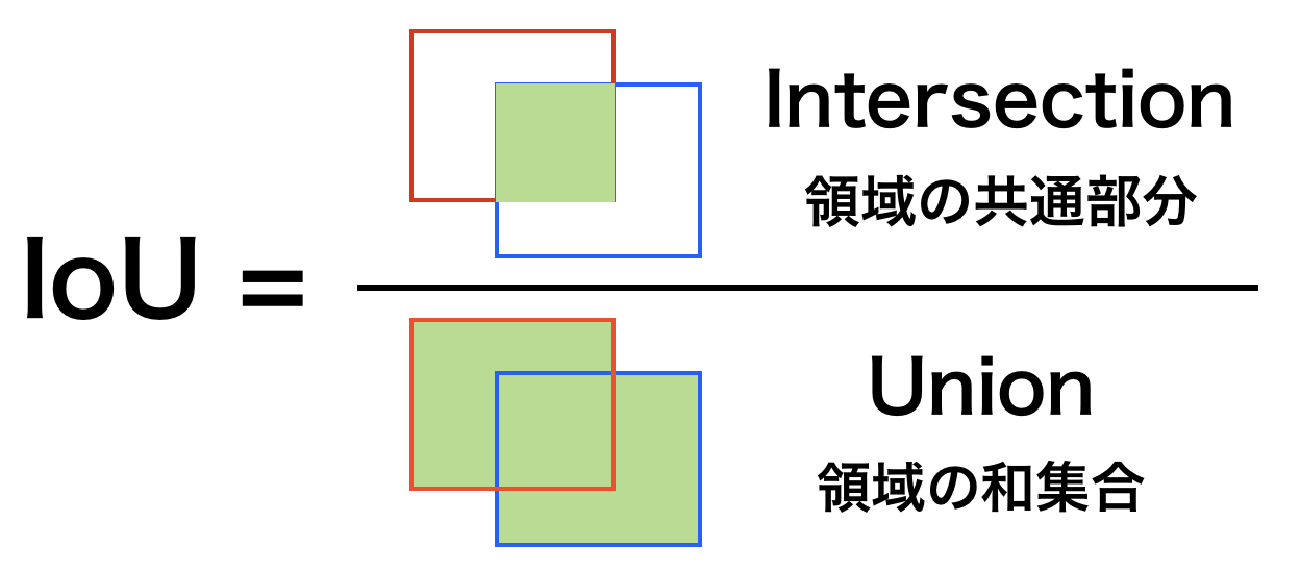
\includegraphics[height=53mm]{iou.eps}
% 	 \caption{Intersection over Union(IOU)}
% 	 \label{fig:f2}
% \end{figure}

% \begin{figure}[htbt]
% 	\centering
% 	 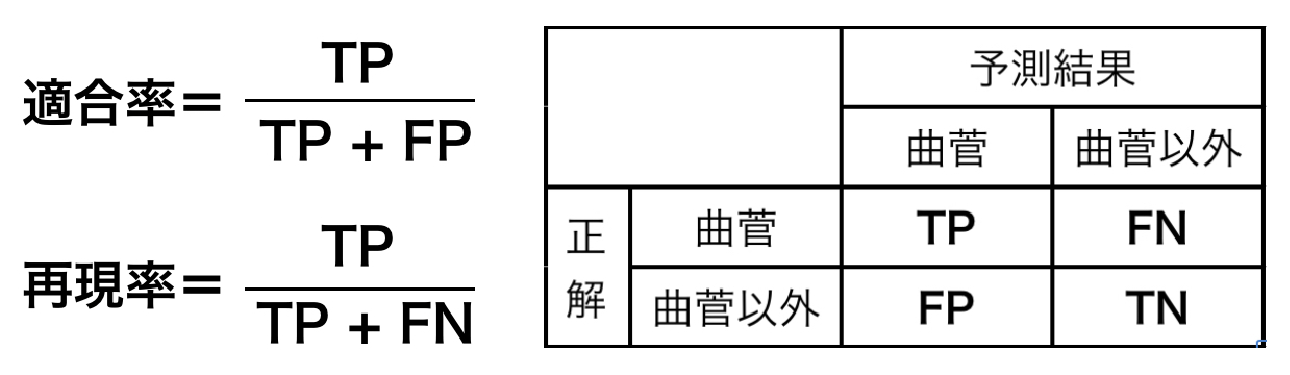
\includegraphics[height=40mm]{recall.eps}
% 	 \caption{適合率と再現率}
% 	 \label{fig:f2}
% \end{figure}

% \section{結果と考察}
% \subsection{物体検出}
% 表3.1,図3.8,図3.9より,RXDネットワークがmAPとmAP50の平均値がともに最も数値が高い結果を示した.APの値が高いほど配管の認識精度が良いことを示しているため,YOLOv3とYOLOv3-DepthよりもRXDネットワークのほうが優れた精度を発揮すると言える.
% また,bentとjunction個々のAP値で見るとYOLOv3よりもRXDのほうがbentを検出するにおいて良い結果を示した.これは曲管を認識する場合,真横からの画角では曲部が再現されず直管のように映し出されることがあるため,RGB画像のみでは直管であると誤認識してしまう恐れがある.
% しかし,Depth画像を用いた場合,曲部が真横からの画角でも奥行きが表現できるため,特徴を捉えやすくなることで認識精度が高い結果になったと考えられる.
% また,評価指標はmAPとmAP50で行ったが,どのネットワークにおいてもmAPのほうがmAP50よりも精度が悪い結果となった.これはmAPの方は閾値を0.5~0.95の間で0.05刻みでIoUの閾値を上昇させているため,重なり合う面積の大きさの条件をより厳しくしているからだ.
% IoU閾値を増加させても認識精度が低くならないネットワークが優秀とされているが,今回の結果においてはどのネットワークも精度が大きく落ちているため,ネットワーク改善を行う必要性があると考えられる.\\
% 次に,パラメータ数に関してはYOLOv3, YOLOv3-DepthよりもRXDは低い値を示している.パラメータ数が高いとネットワークの構造が複雑になることを示しているため,推論時間も比例して長くなる.そのため,RXDは他のネットワークよりも認識結果を
% より速く示すことが期待できる.
% 一方,YOLOv3とYOLOv3-Depthのパラメータ数を比較すると1.4倍ほど差が存在している.YOLOV3-DepthはDepth画像を使用していることからデータセットの量はYOLOv3よりも2倍になるため,ネットワークは必然的に畳み込みむ回数が増加し
% パラメータ数が結果的に多くなることを意味している.そのため,RXDはYOLOv3-Depthと同様にDepth画像を用いていることからパラメータ数が多くなることが予測できるがYOLOv3よりもパラメータ数が低い結果を示した.
% RXDはネットワーク設計段階で畳み込み層の回数の調整や出力チャネルの削減,RXD層の効果的なRGB画像とDepth画像の特徴共有を達成していることがパラメータを数削減しながらも安定した精度を出力する結果につながっていると考えられる.\\




% \clearpage

% \begin{table}[htbp]
% \centering
% \caption{物体検出ネットワークの実行結果}
% \resizebox{\textwidth}{!}{%
% \begin{tabular}{llllllll}
% \hline
% 	\textit{\textbf{}} & \textit{\textbf{}} & \textit{\textbf{mAP}} & \textit{\textbf{}} & \textit{\textbf{}} & \textit{\textbf{mAP50}} & \textit{\textbf{}} & \textit{\textbf{Parameters}} \\
% \textit{\textbf{Network}} & \textit{\textbf{bent}} & \textit{\textbf{junction}} & \textit{\textbf{mean}} &  \textit{\textbf{bent}} & \textit{\textbf{junction}} & \textit{\textbf{mean}} & \textit{\textbf{}} \textit{\textbf{(millions)}} \\ \hline
% YOLOV3              & 33.9                 & 68.6                                 & 51.3                      & 9.95                      & 20.1                          & 15.1                     & 61.5                                \\
% Gen6D      				  & 65.4                 & 34.0                                 & 49.7                      & 19.2                      & 7.6                          	& 13.4                     & 86.3                                	\\
% RXD                 & 70.9                 & 37.2                                 & 54.1                      & 20.8                      & 10.9                          & 15.8                     & 32.4                                 \\
% \end{tabular}%
% }
% \end{table}

% \begin{figure}[htbt]
% 	\centering
% 	 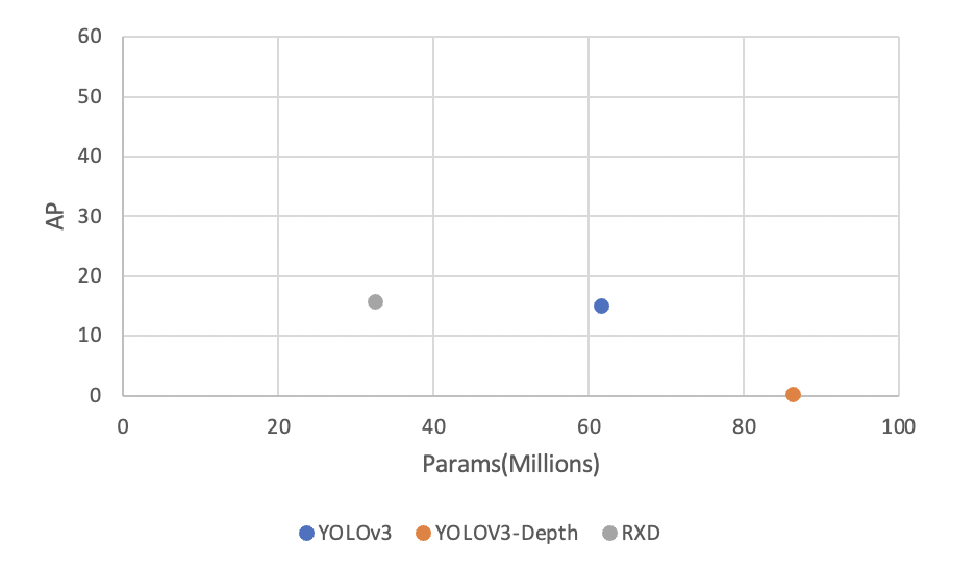
\includegraphics[height=70mm]{ap.eps}
% 	 \caption{mAPによる検出結果}
% 	 \label{fig:f2}
% \end{figure}

% \begin{figure}[htbt]
% 	\centering
	
% 	 \includegraphics[height=70mm]{ap50.eps}
% 	 \caption{mAP50による検出結果}
% 	 \label{fig:f2}
% \end{figure}

% \newpage

% \begin{figure}[htbt]
% 	\centering
% 	 \includegraphics[height=95mm]{re0.eps}
% 	 \label{fig:f2}
% \end{figure}

% \begin{figure}[htbt]
% 	\centering
% 	 \includegraphics[height=95mm]{re1.eps}
% 	 \caption{各ネットワークの検出結果}
% 	 \label{fig:f2}
% \end{figure}

% \newpage

% \clearpage
% \subsection{6D姿勢推定}
% 図3.10にはRGB-Dカメラから得られたRGB画像とDepth画像,曲管やT字管のラベリングを行ったGround Truth画像,各ネットワークの検出結果をそれぞれ示した.結果より正解ラベルと最も近しい検出結果を示したのはRXDネットワークであると言える.
% しかし,RXDネットワークの出力されたデータにはT字管を認識できていない結果も存在している.これは,もとのDepth画像のデータセットを参考にすると遠くの物体になるほどデータが欠落していることが図中の3番の画像からわかる.
% そのため,他のデータセットにおいてもカメラに近いオブジェクトが認識できても遠距離になるにつれて認識精度が悪くなる結果になった.
% よって,精度がより好ましいRGB-Dカメラを使用することや,Depth画像取得の際にフィルタリングでデータの欠落を埋める作業を取り入れる必要性がある.\\
%  また,図中の4番のテスト画像では暗闇の状況下での検出を試みた結果,YOLOv3-DepthとRXDネットワークの出力がうまく配管を検出できていた.
% これは暗闇の状況下でも影響を受けないDepth画像が推論において役に立っていると考えられ,RGB-Dカメラの有効性を示すことができたと言える.

% \begin{figure}[htbt]
% 	\centering
% 	 \includegraphics[height=120mm]{6d.eps}
% 	 \caption{6D姿勢推定の結果}
% 	 \label{fig:f2}
% \end{figure}

% 次に,6D姿勢推定の結果を図3.11に示す.既存のGen6Dのみでは検出器がオブジェクトの複数認識に対応していなかった.RXDネットワークは画像の中の全てのオブジェクトを認識可能なため,検出された値をGen6DのSelectorに渡すことで複数姿勢推定を可能とする.
% しかし,結果では曲管の姿勢がボックスとうまく一致しなく望ましくない結果になったが比較的安定した姿勢推定が行えていると判断できる.

% \begin{table}[htbp]
% \centering
% \caption{それぞれのT字管の姿勢の値}
% \begin{tabular}{llllllll}
% \hline
% \textit{\textbf{}} & \textit{Junction(left)} & \textit{Junction(right)} \\ \hline
% Yaw         & -2.453460 &  0.7020501        \\
% Pitch				&	0.0145083	 &	0.0262553			\\
% Roll        & 1.7120977  & 1.6288774    \\
% \end{tabular}%

% \end{table}

% \begin{figure}[htbt]
% 	\centering
% 	 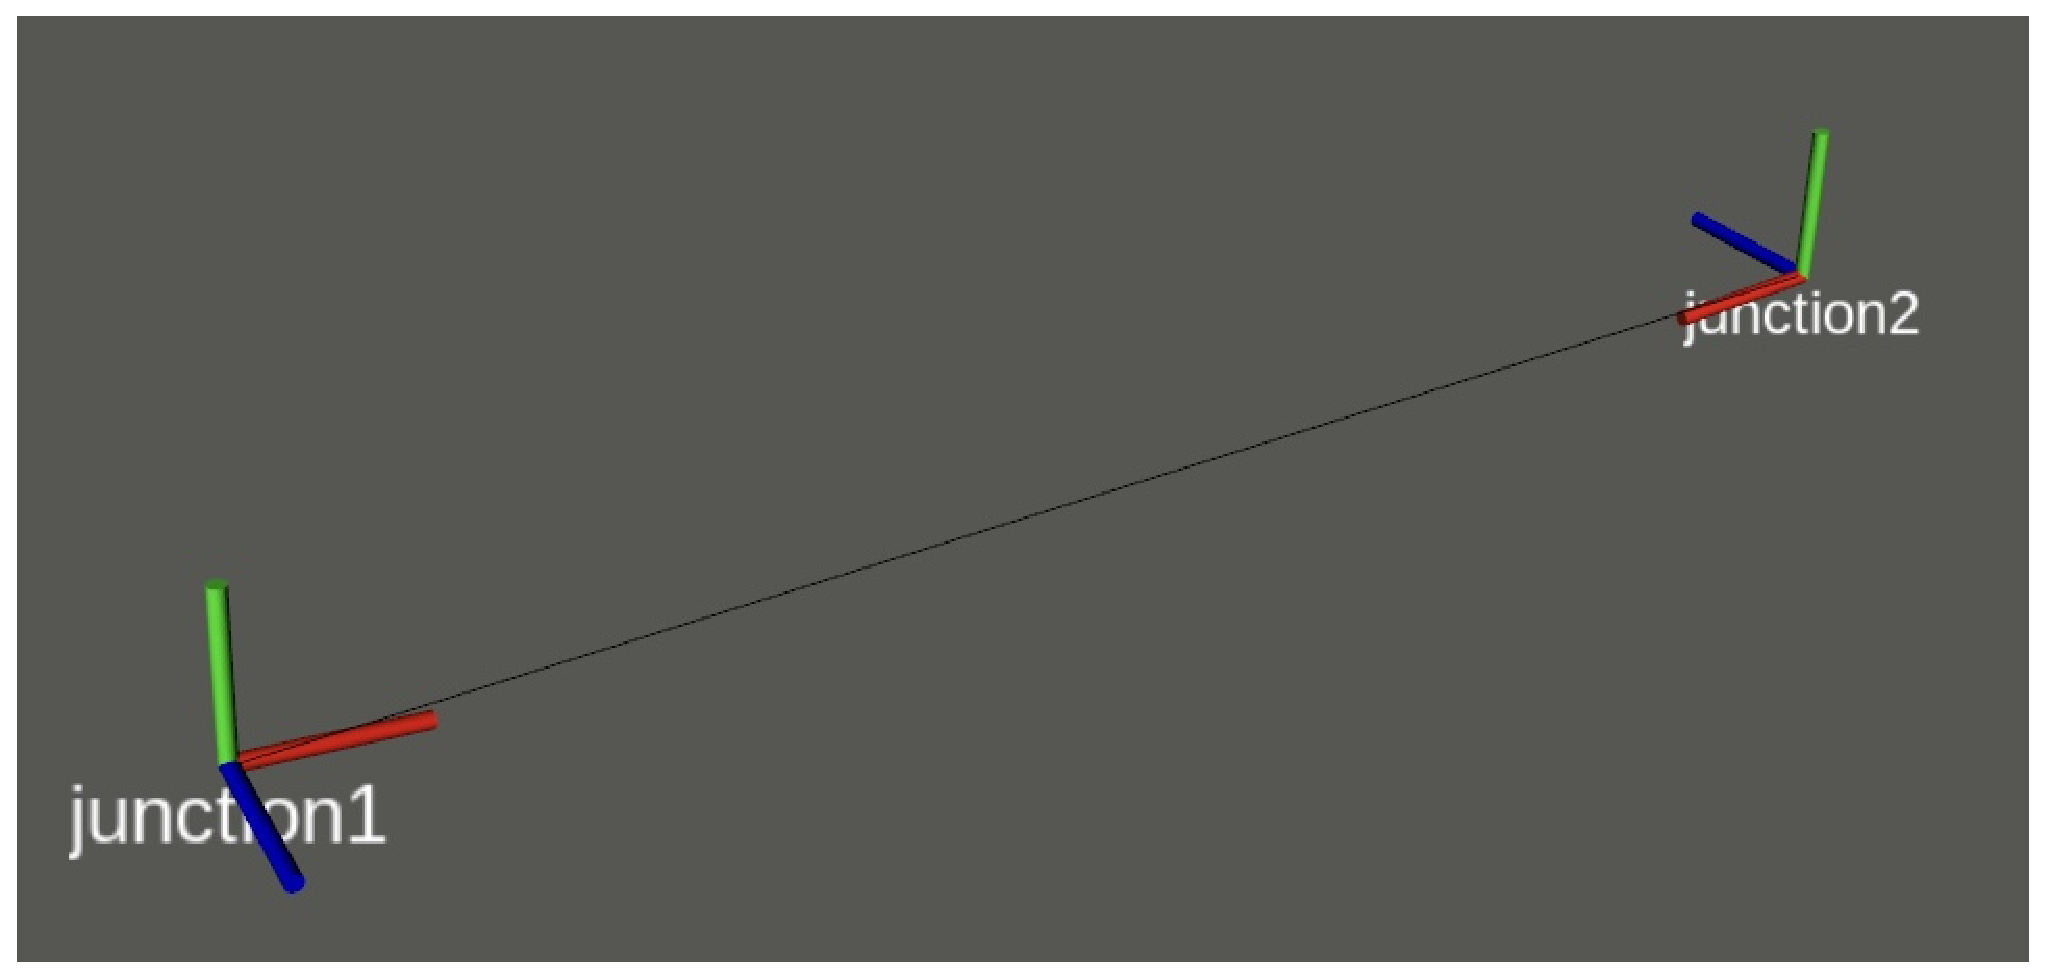
\includegraphics[height=65mm]{rviz.eps}
% 	 \caption{Rvizを用いたT字管の座標系の可視化}
% 	 \label{fig:f2}
% \end{figure}

% また,図3.11の1番の画像のようにjunction同士が向かい合っている画像の姿勢推定より,それぞれのオブジェクトのYaw, Pitch, Rollを求めた.表の結よりjunction同士が向かい合っていることがわかる.
% Gen6Dは認識したオブジェクトに対して回転行列と移動ベクトルを出力する.その結果を元にYaw, Pitch, Rollを算出した.その結果は表3.2のようになり,それぞれの値を用いて,図3.12のようにRvizを使用して
% それぞれのオブジェクトの座標系を可視化した.座標系を求められたことで完全に向かい合った結果にはならなかったが,T字管の位置関係と姿勢を表示することができた.

% \begin{figure}[htbt]
% 	\centering
% 	 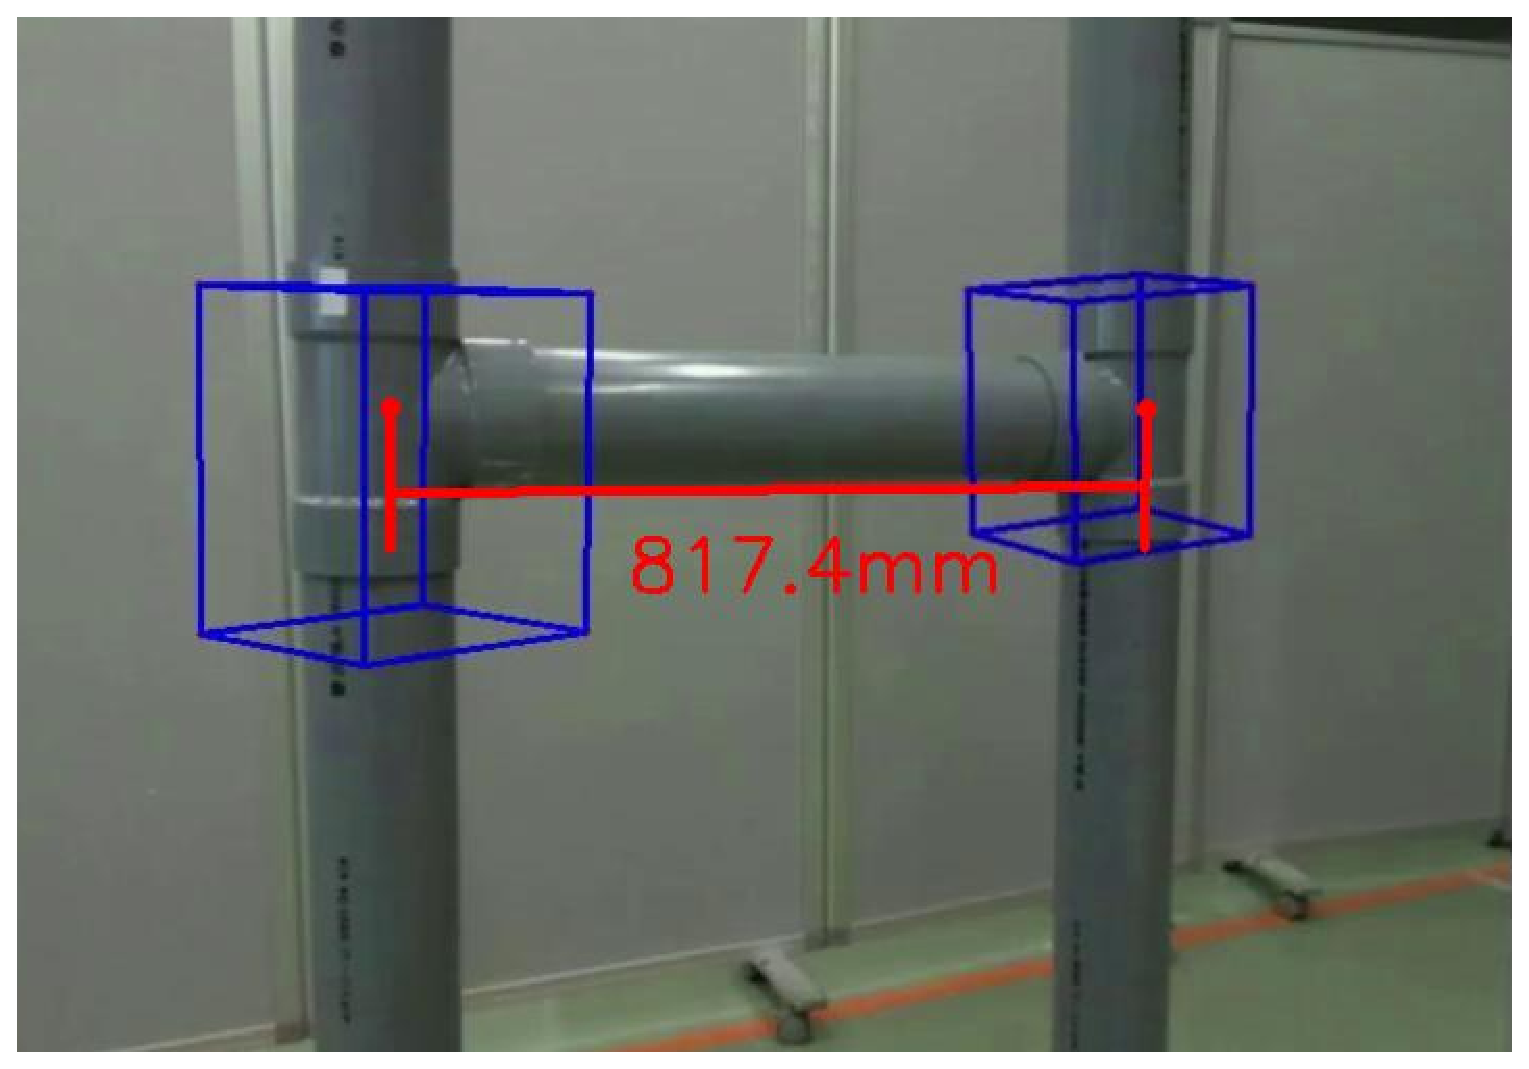
\includegraphics[height=85mm]{scale.eps}
% 	 \caption{算出されたT字管の距離}、
% 	 \label{fig:f2}
% \end{figure}

% \begin{figure}[htbt]
% 	\centering
% 	 \includegraphics[height=85mm]{realscale.eps}
% 	 \caption{実際のT字管の距離}
% 	 \label{fig:f2}
% \end{figure}

% 次に,姿勢推定した結果からDepth画像を使用してT字管の間の距離測定を行う.姿勢推定した結果には距離情報を含んでいないため,推定されたオブジェクトのピクセル中心座標を深度画像と照らし合わせることでオブジェクト間の距離を算出する.
% 図3.13及び図3.14にそれぞれに実際の測定値と出力された結果を用いて算出された距離情報の結果を示す.実際の距離が817.3mmだったのに対し,Depth画像によって求められたスケールは817.3mmであった.誤差は生じているが,Depth画像を用いることで
% 姿勢推定した結果に距離情報を与えることができていると言える.ただし図3.14では正確な距離を取得できないため,実際に寸法を図る際は地面においた状態で測定した.\\
% \clearpage
% \begin{figure}[htbt]
% 	\centering
% 	 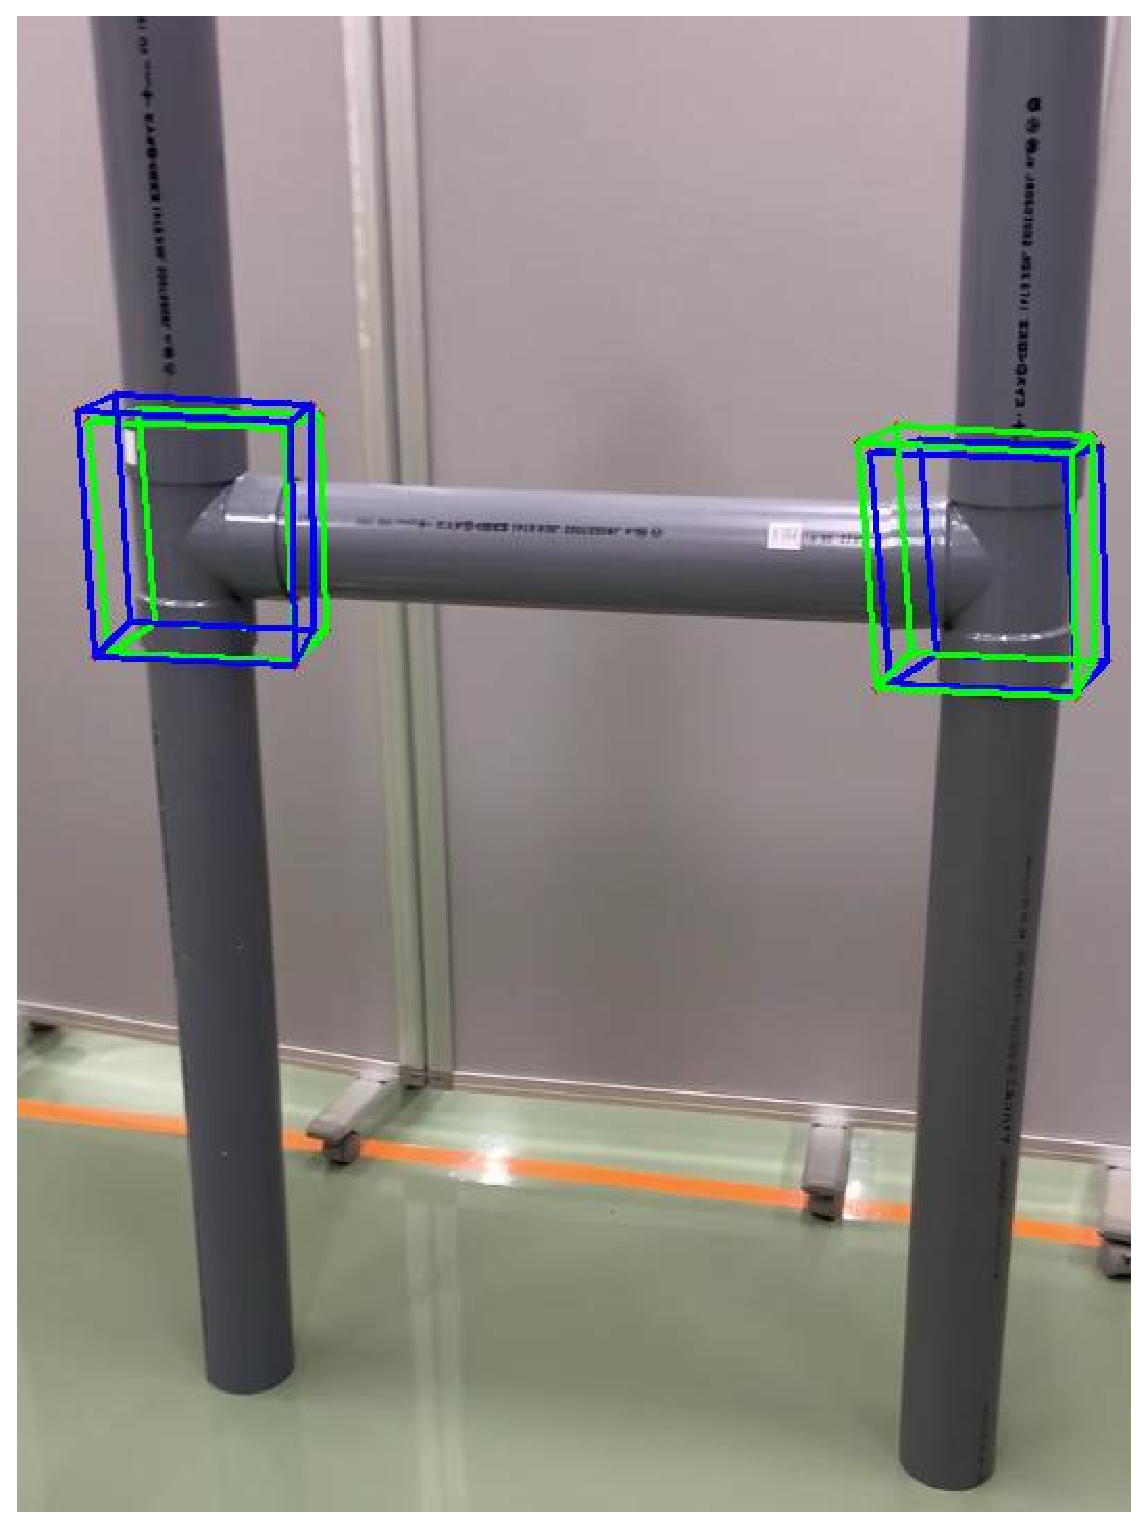
\includegraphics[height=120mm]{test6.eps}
% 	 \caption{テストデータを用いた姿勢推定の例}
% 	 \label{fig:f2}
% \end{figure}

% \begin{table}[htbp]
% \centering
% \caption{6D姿勢推定の評価}
% \begin{tabular}{llllllll}
% \hline
% % \textit{\textbf{}} & \textit{bent} & \textit{junction} & \textit{mean} \\ \hline
% % ADD-0.1d        & 26.35 & 46.54 & 36.445 \\
% % Prj-5				&	72.64	 &	89.32	& 80.98		\\
% \textit{\textbf{}} & \textit{Gen6D} & \textit{RXD} \\ \hline
% ADD-0.1d        & 26.35  & 36.445 \\
% Prj-5				&	72.64 &	 80.98		\\
% \end{tabular}%
% \end{table}
% 最後に,図3.15のようにテストデータを用いた姿勢推定の精度評価を行った.推測データを青色のバウンディングボックス,正解データを緑色のバウンディングボックスを示した.
% また表3.3より,複数のテストデータで行い,曲管とT字管それぞれの姿勢の値を精度評価した.曲管よりもT字管の推論値のほうが正確に判断できた結果となった.これは曲管の姿勢推定を行う場合,
% 真正面からの画角では曲部が鮮明に映し出されるが,真横からの画角では曲管が直管のように直線であるかのように誤認識されてしまうことが原因で認識精度が落ちている.
% そのため,6D姿勢推定においてもDepth画像を使用し2D画像では認識できない奥行き情報を使用することでより推論データの精度も向上すると考えられる.
% 以上の結果より,アイソメ図作成に必要な情報である曲管及びT字管の姿勢推定と距離情報を求められるプロセスを確立することができた.

